\documentclass[
    10pt,
    aspectratio=169,
    xcolor={dvipsnames},
    spanish,
    % handout,
    % notes=only,
    % notes,
    ]{beamer}

% BEAMER SETTINGS
\setbeamerfont{section in toc}{size=\normalsize, shape=\bfseries}
\mode<presentation>{
    \usetheme{Antibes}
    \setbeamercovered{transparent}
    \usecolortheme{rose}
    \setbeamertemplate{navigation symbols}{}
    }
\useoutertheme{infolines}

% PACKAGES
\usepackage[spanish]{babel}  % Spanish support enabled
\usepackage{tikz,pgfplots}
\pgfplotsset{compat=1.13}
\usetikzlibrary{calc}
\usepackage{subcaption}
\usepackage{graphicx}
\graphicspath{{figures}}
\usepackage{booktabs}
\usepackage{upgreek}
\usepackage{commath}
\usepackage{amsmath,amsthm,amssymb,mathtools,mathrsfs}
\usepackage{cancel}
\usepackage{fontawesome5}
\usepackage{enumerate}
\usepackage{tensor}
\usepackage[font=footnotesize]{caption}
\usepackage{wasysym}

\usepackage[skins,theorems]{tcolorbox}
\tcbset{
    highlight math style={
        enhanced,
        coltext=black,
        colframe=black,
        colback=lightgray,
        arc=0pt,
        boxrule=.5pt
        }
}

% REFERENCES AND OTHERS
\usepackage{aas_macros}
\usepackage{natbib}
\bibpunct{(}{)}{;}{a}{}{,}

\usepackage{siunitx}
\sisetup{
    range-phrase=\text{--},
    range-units=single,
    separate-uncertainty=true,
    print-unity-mantissa=false
    }
\DeclareSIUnit{\gauss}{G}
\DeclareSIUnit{\jansky}{Jy}
\renewcommand{\figurename}{Fig.}

\usepackage{hyperref}
\hypersetup{
    % bookmarks=true,
    unicode=true,
    pdftoolbar=true,
    pdfmenubar=true,
    pdffitwindow=false,
    pdfstartview={FitH},
    pdftitle={ISI-Free Linear Combination Pulses with Better Performanc},
    pdfauthor={Erik Saez A.},
    pdfcreator={Erik Saez A.},
    pdfnewwindow=true,
    colorlinks=true,
    linkcolor=RoyalBlue,
    citecolor=RoyalBlue,
    urlcolor=RoyalBlue
    }

\title[Auxiliar \#2 - Semiconductores]{\bfseries Auxiliar \#2 - Semiconductores}
\subtitle{Circuitos Eléctricos Analógicos (EL3202-1)}
\author[Erik Saez A.]{Erik Saez A.}
\institute[UChile]{Department of Electrical Engineering \\ Universidad de Chile}

\date{\today}

\begin{document}

\begin{frame}
  \titlepage
  \centering
  \faIcon{envelope} \href{mailto:erik.saez@ug.uchile.cl}{erik.saez@ug.uchile.cl} \hspace{.2cm}
\end{frame}

\begin{frame}
  \frametitle{Contenidos}
  \centering
  \begin{columns}
    \begin{column}{0.4\textwidth}
      \tableofcontents
    \end{column}
    \begin{column}{0.5\textwidth}
      \begin{figure}
        \centering
        
\includegraphics[width=\textwidth]{fcfm_die}
        \caption{Facultad de Ciencias Físicas y Matemáticas, Universidad de Chile.}
      \end{figure}
    \end{column}
  \end{columns}  
\end{frame}
%%%%%%%%%%%%%%%%%%%%%%%%%%%%%%%%%%%%%%%%%%

\section{Resumen}

\begin{frame}{Impurezas en Semiconductores}
\begin{block}{Conceptos Fundamentales}
  \begin{itemize}
    \item 	\textbf{Semiconductores puros}: Silicio (Si) y Germanio (Ge) - Grupo IV con 4 electrones de valencia
    \item 	\textbf{Dopaje}: Proceso de añadir impurezas intencionalmente para modificar propiedades eléctricas
    \item 	\textbf{Propósito}: Controlar la conductividad y crear dispositivos electrónicos
  \end{itemize}
\end{block}

\begin{columns}
  \begin{column}{0.48\textwidth}
    \begin{block}{Impurezas Donadoras (Tipo N)}
      \scriptsize
      \begin{itemize}
        \item 	\textbf{Origen}: Grupo V (P, As, Sb) - 5 electrones de valencia
        \item 	\textbf{Mecanismo}: 4 electrones forman enlaces, 1 queda libre
        \item 	\textbf{Resultado}: Electrón libre + ion donador positivo fijo
        \item 	\textbf{Portadores mayoritarios}: Electrones (en banda de conducción)
      \end{itemize}
    \end{block}
  \end{column}

  \begin{column}{0.48\textwidth}
    \begin{block}{Impurezas Aceptoras (Tipo P)}
      \scriptsize
      \begin{itemize}
        \item 	\textbf{Origen}: Grupo III (B, Al, Ga) - 3 electrones de valencia
        \item 	\textbf{Mecanismo}: Forman solo 3 enlaces, dejan 1 incompleto
        \item 	\textbf{Resultado}: Hueco + ion aceptor negativo fijo
        \item 	\textbf{Portadores mayoritarios}: Huecos (en banda de valencia)
      \end{itemize}
    \end{block}
  \end{column}
\end{columns}
\end{frame}
%-----------------------------------------
\begin{frame}
  \begin{figure}
    \centering
    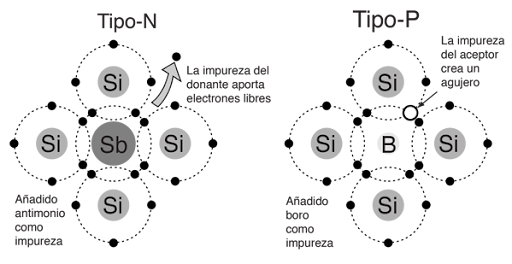
\includegraphics[width=0.8\textwidth]{../figures/Auxiliar_2_13.png}
    \caption{Diagrama de bandas en un semiconductor tipo p-n}
  \label{fig:bandas_polarizacion}
\end{figure}
\end{frame}
%%%%%%%%%%%%%%%%%%%%%%%%
\begin{frame}{Ley de Acción de Masas}
\begin{columns}
  \begin{column}{0.48\textwidth}
    \begin{block}{Ecuación Fundamental}
      \footnotesize
      Para cualquier semiconductor en equilibrio térmico:
      \begin{equation}
        n_0 \cdot p_0 = n_i^2 \tag{Ley de Acción de Masas}
      \end{equation}
      \textbf{Donde:}
      \begin{itemize}
        \item $n_0$: Concentración de electrones [cm$^{-3}$]
        \item $p_0$: Concentración de huecos [cm$^{-3}$] 
        \item $n_i$: Concentración intrínseca [cm$^{-3}$]
      \end{itemize}
    \end{block}
  \end{column}
  
  \begin{column}{0.48\textwidth}
    \begin{block}{Características Importantes}
      \footnotesize
      Esta relación es fundamental porque:
      \begin{enumerate}
        \item Es válida para semiconductores intrínsecos y dopados
        \item Se cumple en equilibrio térmico
        \item Permite calcular una concentración conociendo la otra
        \item Es independiente del tipo de dopaje
      \end{enumerate}
    \end{block}
  \end{column}
\end{columns}

\begin{block}{Aproximaciones Útiles para Dopaje Fuerte}
  \footnotesize
  \begin{columns}
    \begin{column}{0.48\textwidth}
      \textbf{Material tipo N} ($N_d \gg n_i$):
      \begin{equation}
        n_0 \approx N_d \quad \text{y} \quad p_0 \approx \frac{n_i^2}{N_d}
      \end{equation}
    \end{column}

    \begin{column}{0.48\textwidth}
      \textbf{Material tipo P} ($N_a \gg n_i$):
      \begin{equation}
        p_0 \approx N_a \quad \text{y} \quad n_0 \approx \frac{n_i^2}{N_a}
      \end{equation}
    \end{column}
  \end{columns}
\end{block}
\end{frame}
%------------------------------
%%%%%%%%%%%%%%%%%%%%%%%%
\begin{frame}{Nivel de Fermi y Bandas de Energía}
\begin{columns}
  \begin{column}{0.55\textwidth}
    \begin{block}{Nivel de Fermi ($E_F$)}
      \scriptsize
      \textbf{Definición}: Nivel energético que separa estados ocupados de vacíos a T = 0K. A temperaturas finitas, se suaviza según la distribución de Fermi-Dirac.

      \vspace{0.3cm}
      \textbf{Comportamiento según dopaje:}
      \begin{itemize}
        \item \textbf{Intrínseco}: $E_F \approx E_i$ (centro del gap)
        \item \textbf{Tipo N}: $E_F > E_i$ (hacia banda conducción)
        \item \textbf{Tipo P}: $E_F < E_i$ (hacia banda valencia)
      \end{itemize}
    \end{block}
  \end{column}
  
  \begin{column}{0.43\textwidth}
    \begin{block}{Generación Térmica}
      \scriptsize
      En semiconductores intrínsecos a $T > 0$:
      \begin{itemize}
        \item Energía térmica $kT$ excita electrones
        \item Electrones saltan de banda valencia a conducción
        \item Se crean pares electrón-hueco simultáneamente
        \item $n_0 = p_0 = n_i$ (neutralidad de carga)
      \end{itemize}
    \end{block}
  \end{column}
\end{columns}
  \begin{figure}[H]
    \centering
    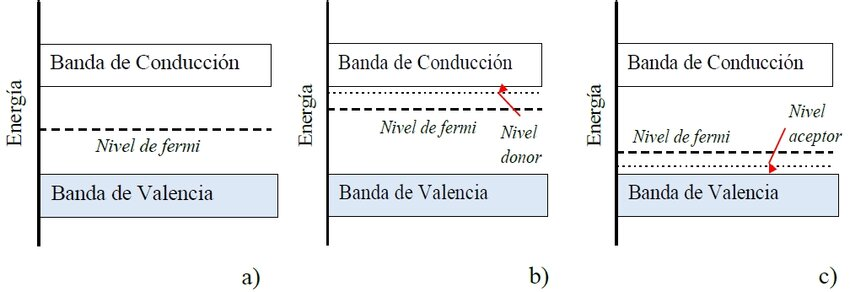
\includegraphics[width=0.6\textwidth]{../figures/Auxiliar_2_5.jpg}
    \caption{Niveles de Fermi para diferentes dopajes.}
  \label{fig:bandas_polarizacion}
\end{figure}
\end{frame}

%%%%%%%%%%%%%%%%%%%%%%%%
\begin{frame}{Corriente de Difusión}
\begin{block}{Concepto y Ecuaciones Fundamentales}
  \footnotesize
  La corriente de difusión se genera por el movimiento de portadores desde regiones de alta concentración hacia regiones de baja concentración.
  
  \vspace{0.2cm}
  \textbf{Para electrones:}
  \begin{equation}
    J_n = eD_n \frac{dn}{dx}
  \end{equation}
  
  \textbf{Para huecos:}
  \begin{equation}
    J_p = -eD_p \frac{dp}{dx}
  \end{equation}
\end{block}

\begin{columns}
  \begin{column}{0.48\textwidth}
    \begin{block}{Variables del Sistema}
      \scriptsize
      \begin{itemize}
        \item $e$: Carga elemental ($1{,}6 \times 10^{-19}$ C)
        \item $D_n, D_p$: Coeficientes de difusión [cm$^2$/s]
        \item $\frac{dn}{dx}, \frac{dp}{dx}$: Gradientes de concentración [cm$^{-4}$]
        \item $J_n, J_p$: Densidades de corriente [A/cm$^2$]
      \end{itemize}
    \end{block}
  \end{column}
  
  \begin{column}{0.48\textwidth}
    \begin{block}{Condición: Dopaje Uniforme}
      \scriptsize
      Si la concentración es constante espacialmente:
      \begin{itemize}
        \item $\frac{dn}{dx} = 0$ y $\frac{dp}{dx} = 0$
        \item Resultado: $J_n = 0$ y $J_p = 0$
        \item \textbf{No hay corriente de difusión}
        \item Solo existe corriente de deriva (campo eléctrico)
      \end{itemize}
    \end{block}
  \end{column}
\end{columns}
\end{frame}

%%%%%%%%%%%%%%%%%%%%%%%%
%%%%%%%%%%%%%%%%%%%%%%%%
\begin{frame}{Unión p-n: Conceptos Fundamentales}
\begin{columns}
  \begin{column}{0.48\textwidth}
    \begin{block}{Formación de la Unión (V = 0)}
      \scriptsize
      En equilibrio térmico sin voltaje externo:
      \begin{itemize}
        \item \textbf{Difusión inicial}: Electrones van de n $\rightarrow$ p, huecos van de p $\rightarrow$ n
        \item \textbf{Región de depleción}: Se forman iones fijos ($N_d^+$ y $N_a^-$)
        \item \textbf{Campo eléctrico interno}: Opone la difusión
        \item \textbf{Equilibrio}: Difusión = Deriva (corriente neta = 0)
        \item \textbf{Voltaje de contacto}: $V_0 = V_T \ln\left(\frac{N_a N_d}{n_i^2}\right)$
      \end{itemize}
    \end{block}
  \end{column}
  
  \begin{column}{0.48\textwidth}
    \begin{block}{Efectos de Polarización Externa}
      \scriptsize
      \textbf{Polarización Directa} ($V > 0$):
      \begin{itemize}
        \item Reduce la barrera de potencial
        \item Facilita flujo de portadores mayoritarios
        \item Corriente exponencial: $I \propto e^{V/V_T}$
      \end{itemize}
      
      \vspace{0.2cm}
      \textbf{Polarización Inversa} ($V < 0$):
      \begin{itemize}
        \item Aumenta la barrera de potencial
        \item Bloquea portadores mayoritarios
        \item Solo corriente de saturación inversa
      \end{itemize}
    \end{block}
  \end{column}
\end{columns}

\begin{block}{Concentraciones en Equilibrio}
  \scriptsize
  \begin{columns}
    \begin{column}{0.24\textwidth}
      \textbf{Región tipo N:}
      \begin{align}
        n_n &\approx N_d \\
        p_n &= \frac{n_i^2}{N_d}
      \end{align}
    \end{column}
    
    \begin{column}{0.24\textwidth}
      \textbf{Región tipo P:}
      \begin{align}
        p_p &\approx N_a \\
        n_p &= \frac{n_i^2}{N_a}
      \end{align}
    \end{column}

    \begin{column}{0.48\textwidth}
      \textbf{Donde:} $V_T = \frac{kT}{e} \approx 26\,\text{mV}$ a temperatura ambiente (293 K). El nivel de Fermi se alinea a través de la unión en equilibrio, como se muestra en la figura.
    \end{column}
  \end{columns}
\end{block}
\end{frame}

\begin{frame}
    \begin{figure}[H]
    \centering
    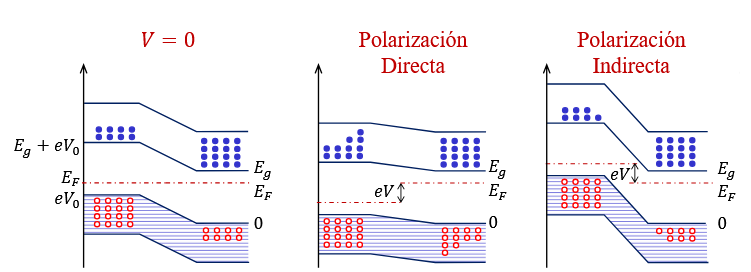
\includegraphics[width=0.8\textwidth]{../figures/Auxiliar_2_14.png}
    \caption{Diagramas de bandas para unión p-n: (izquierda) equilibrio térmico V=0, (centro) polarización directa, (derecha) polarización inversa. Se observa cómo el voltaje externo modifica la curvatura de las bandas y el flujo de portadores.}
  \label{fig:bandas_polarizacion}
\end{figure}
\end{frame}
%=================================
\section{Pregunta 1}
\begin{frame}{Ejercicio}
\begin{block}{Enunciado}
\begin{enumerate}
    \item Explique qué son las impurezas donadoras y las impurezas aceptoras.
    \item ¿A qué es igual el producto de $n_0$ y $p_0$?
    \item ¿De dónde provienen los huecos y electrones en un semiconductor para el caso intrínseco?
    \item Explique cómo se mueve la posición de la Energía de Fermi según se dope un semiconductor con átomos aceptores o átomos donadores.
    \item ¿Qué es la corriente de difusión? ¿Por qué esta corriente es $0$ si se dopa uniformemente un semiconductor?
\end{enumerate}
\end{block}
\end{frame}
%=================================
\begin{frame}
  \begin{block}{Resolución 1.1}
    Explique qué son las impurezas donadoras y las impurezas aceptoras.
  \end{block}
  \begin{figure}
    \centering
    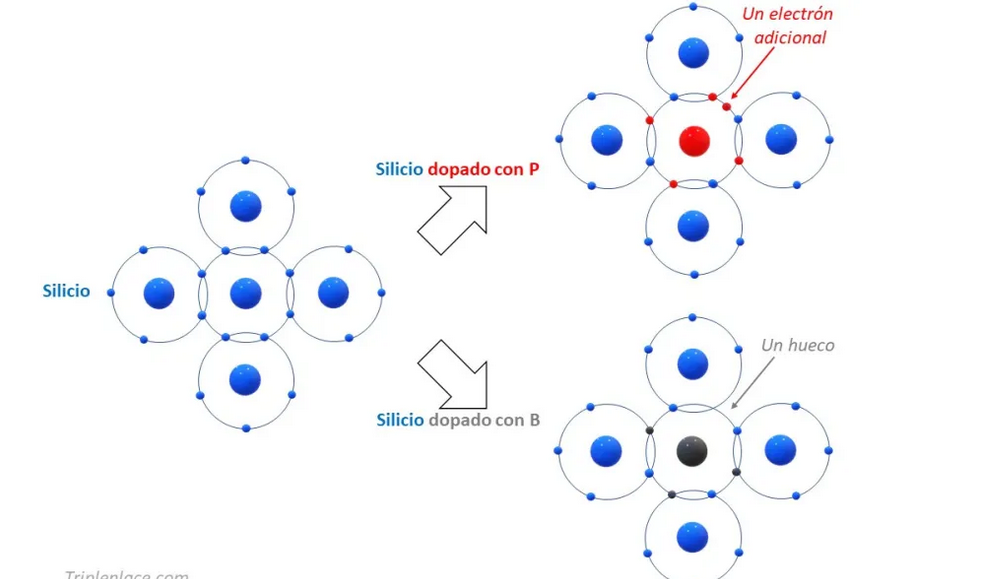
\includegraphics[width=0.6\textwidth]{../figures/Auxiliar_2_3.png}
    \caption{Representación atómica del silicio puro y dopado. Se muestra: (izquierda) silicio puro con enlaces covalentes completos, (arriba derecha) silicio dopado con fósforo (P) donde se observa un electrón adicional libre, y (abajo derecha) silicio dopado con boro (B) donde se forma un hueco por la falta de un electrón en el enlace covalente}
  \end{figure}
\end{frame}

%===================================
\begin{frame}
  \begin{block}{Resolucion 1.2}
    ¿A qué es igual el producto de $n_0$ y $p_0$?
  \end{block}
  
  \begin{columns}
    \begin{column}{0.48\textwidth}
      \begin{block}{Ley de Acción de Masas}
        \footnotesize
        El producto de concentraciones está dado por:
        \begin{equation}
          n_0 p_0 = n_i^{2}  
        \end{equation}
        
        \textbf{Variables:}
        \begin{itemize}
          \item $n_0$: Concentración de electrones en equilibrio [cm$^{-3}$]
          \item $p_0$: Concentración de huecos en equilibrio [cm$^{-3}$]
          \item $n_i$: Concentración intrínseca [cm$^{-3}$]
        \end{itemize}
      \end{block}
    \end{column}
    
    \begin{column}{0.48\textwidth}
      \begin{block}{Importancia}
        \footnotesize
        Esta relación es fundamental porque:
        \begin{enumerate}
          \item Válida para semiconductores intrínsecos y dopados
          \item Se cumple en equilibrio térmico
          \item Permite calcular una concentración conociendo la otra
        \end{enumerate}
      \end{block}
    \end{column}
  \end{columns}

  \begin{block}{Método de Cálculo para Dopaje Fuerte}
    \footnotesize
    \begin{columns}
      \begin{column}{0.48\textwidth}
        \textbf{Material tipo N} (impurezas donadoras):
        \begin{equation}
          n_0 \approx N_d \quad \text{y} \quad p_0 \approx \frac{n_i^2}{N_d}
        \end{equation}
      \end{column}
      
      \begin{column}{0.48\textwidth}
        \textbf{Material tipo P} (impurezas aceptoras):
        \begin{equation}
          p_0 \approx N_a \quad \text{y} \quad n_0 \approx \frac{n_i^2}{N_a}
        \end{equation}
      \end{column}
    \end{columns}
  \end{block}
\end{frame}
%--------------------------------
\begin{frame}
  \begin{block}{Resolucion 1.3}
    De donde provienen los huecos y electrones en un semiconductor para el caso intrínseco?
  \end{block}
    \begin{figure}
    \centering
    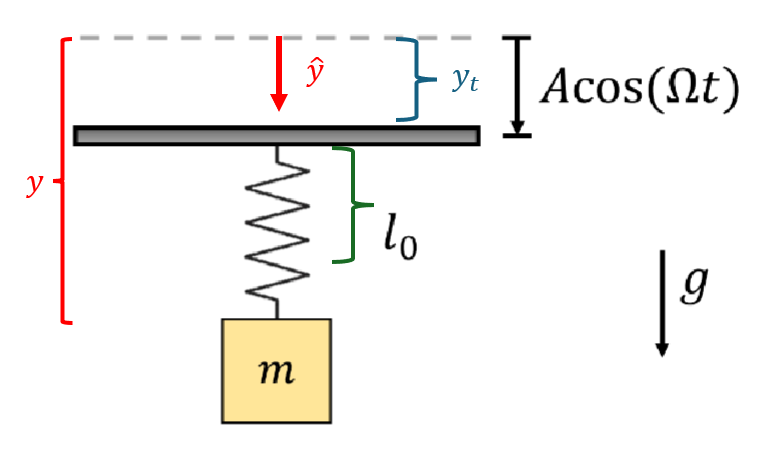
\includegraphics[width=0.45\textwidth]{../figures/Auxiliar_2_4.png}
    \caption{Generación térmica de pares electrón-hueco en un semiconductor intrínseco. (Izquierda) Representación atómica mostrando un electrón (azul) que absorbe energía térmica y se libera de un enlace covalente. (Derecha) Diagrama de bandas de energía ilustrando cómo un electrón supera el gap energético para pasar de la banda de valencia a la banda de conducción, dejando un hueco en la banda de valencia.}
  \end{figure}
\end{frame}
%----------------------------------------
\begin{frame}
  \begin{block}{Resolucion 1.4}
   Explique cómo se mueve la posición de la Energía de Fermi según se dope un semiconductor con átomos aceptores o átomos donadores.
  \end{block}
  
  \begin{columns}
    \begin{column}{0.5\textwidth}
      \begin{figure}
        \centering
        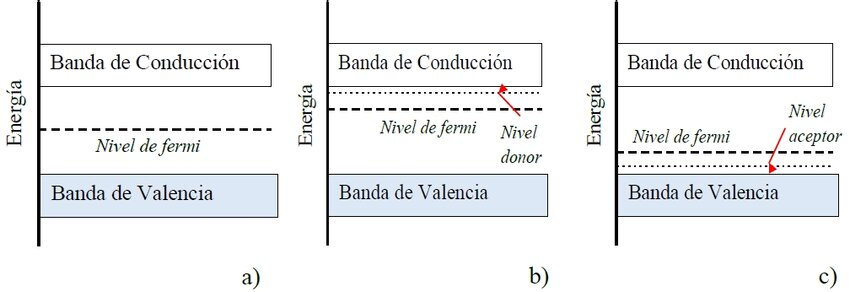
\includegraphics[width=\textwidth]{../figures/Auxiliar_2_5}
        \caption{Diagrama de bandas de energía mostrando la posición del nivel de Fermi.}
        \label{fig:fermi}
      \end{figure}
    \end{column}
    
    \begin{column}{0.48\textwidth}
      \begin{block}{Posición del Nivel de Fermi}
        \scriptsize
        Como se observa en la Figura \ref{fig:fermi}:
        
        \vspace{0.2cm}
        \textbf{a) Semiconductor intrínseco:}
        \begin{itemize}
          \item $E_F \approx E_i$ (centro del gap)
          \item $n_0 = p_0 = n_i$
        \end{itemize}
        
        \vspace{0.2cm}
        \textbf{b) Tipo N (donadores):}
        \begin{itemize}
          \item $E_F > E_i$ (hacia banda conducción)
          \item $n_0 > p_0$
          \item Niveles donadores cerca de BC
        \end{itemize}
        
        \vspace{0.2cm}
        \textbf{c) Tipo P (aceptores):}
        \begin{itemize}
          \item $E_F < E_i$ (hacia banda valencia)
          \item $p_0 > n_0$
          \item Niveles aceptores cerca de BV
        \end{itemize}
      \end{block}
    \end{column}
  \end{columns}
\end{frame}
\begin{frame}
  \begin{block}{Resolucion 1.5}
    ¿Qué es la corriente de difusión? ¿Por qué esta corriente es $0$ si se dopa uniformemente un semiconductor?
  \end{block}
  
  \begin{columns}
    \begin{column}{0.5\textwidth}
      \begin{block}{Definición}
        \scriptsize
        La corriente de difusión se genera por el movimiento de portadores desde regiones de alta concentración hacia regiones de baja concentración.
        
        \vspace{0.3cm}
        \textbf{Ecuaciones fundamentales:}
        
        Para electrones:
        \begin{equation}
          J_n = eD_n \frac{dn}{dx}
        \end{equation}
        
        Para huecos:
        \begin{equation}
          J_p = -eD_p \frac{dp}{dx}
        \end{equation}
      \end{block}
    \end{column}
    
    \begin{column}{0.48\textwidth}
      \begin{block}{Variables}
        \scriptsize
        \begin{itemize}
          \item $J_n, J_p$: densidad de corriente [A/cm$^2$]
          \item $e$: carga elemental ($1{,}6 \times 10^{-19}$ C)
          \item $D_n, D_p$: coeficientes de difusión [cm$^2$/s]
                    \item $\frac{dn}{dx}, \frac{dp}{dx}$: gradientes de concentración [cm$^{-4}$]
        \end{itemize}
      \end{block}
      
      \begin{block}{Caso Especial: Dopaje Uniforme}
        \scriptsize
        Si la concentración es constante espacialmente:
        \begin{itemize}
          \item $\frac{dn}{dx} = 0$ y $\frac{dp}{dx} = 0$
          \item Resultado: $J_n = 0$ y $J_p = 0$
          \item \textbf{No hay corriente de difusión}
          \item Solo existe corriente de deriva por campo eléctrico
        \end{itemize}
      \end{block}
    \end{column}
  \end{columns}

  \begin{block}{Conclusión}
    \scriptsize
    La corriente de difusión solo existe cuando hay variaciones espaciales (gradientes) en las concentraciones de portadores. En materiales uniformemente dopados, no hay gradientes y por tanto no hay corriente de difusión.
  \end{block}
\end{frame}
%%%%%%%%%%%%%%%%%%%%%%
\section{Ejercicio 2}
\begin{frame}{Enunciado 2}
  \begin{block}{Enuncado 2}
Calcule las concentraciones de huecos y electrones en un material semiconductor de silicio que tiene una concentración intrínseca de $n_i = 10^{10}\,\text{cm}^{-3}$, cuando este material se encuentra a una temperatura de $293^\circ \text{K}$. Explicite en qué banda de energía se encuentra respectivamente cada tipo de partícula (hueco o electrón).
  \end{block}
\end{frame}
%----------------------------
\begin{frame}
      \begin{figure}[H]
        \centering
        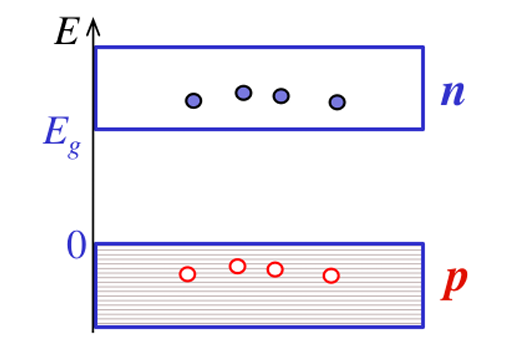
\includegraphics[width=0.6\textwidth]{../figures/Auxiliar_2_6}
        \caption{Bandas de energía en un semiconductor intrínseco con temperatura mayor que cero. Se observan electrones (círculos azules) en la banda de conducción y huecos (círculos rojos) en la banda de valencia debido a la excitación térmica.}
        \label{fig:bandas_temp}
    \end{figure}
\end{frame}
%---------------------------
\section{Ejercicio 3}
\begin{frame}{Enunciado 3}
  \begin{block}{Enunciado 3}
    Un material semiconductor está formado principalmente de silicio, con concentración intrínseca de $n_i = 10^{10}\,\text{cm}^{-3}$, pero dopado con partículas de fósforo con una concentración de $10^{17}\,\text{cm}^{-3}$. Cuando este material se encuentra a una temperatura de $293^\circ \text{K}$:
\begin{itemize}
    \item Calcule las concentraciones de huecos y electrones utilizando el método exacto.
    \item Calcule las concentraciones de huecos y electrones utilizando el método aproximado.
    \item ¿Cuál es el error cometido al aproximar? ¿Qué ecuación no se cumple al hacer la aproximación?
    \item Explicite en qué banda de energía se encuentran respectivamente cada tipo de partícula (hueco o electrón).
    \item ¿Qué tipo de material es este semiconductor?
\end{itemize}
\end{block}
\end{frame}
%---------------------------
\section{Ejercicio 4}
\begin{frame}{Enunciado 4}
  \begin{block}{Enunciado 4}
  Un material semiconductor está formado principalmente de silicio pero que ha sido dopado en una parte con moléculas de Boro (parte gris de la Figura \ref{fig:concentraciones_pn}) con una concentración de $10^{16}\,\text{cm}^{-3}$ y dopado con partículas de fósforo con una concentración de $10^{17}\,\text{cm}^{-3}$ (parte blanca de la Figura \ref{fig:concentraciones_pn}). Recuerde que el silicio tiene una concentración intrínseca de $n_i = 10^{10}\,\text{cm}^{-3}$ cuando este material se encuentra operando a una temperatura de $293^\circ \text{K}$.

\begin{enumerate}
    \item ¿Qué tipo de materiales son cada parte dopada diferente?
    \item ¿Cuáles son las concentraciones de equilibrio en este material?
    \item ¿Existe un voltaje entre los dos tipos de materiales? Si es así, ¿cuál es el valor?
    \item ¿Qué representan las curvas verdes y azules en la Figura?, ¿qué representan la Abscisa y la Ordenada en la figura?
    \item Bosqueje un diagrama de bandas de energía para esta situación.
\end{enumerate}
\end{block}
\end{frame}
%%%%%%%%%%%%%%%%%%%%%%  
\begin{frame}
  \begin{figure}[H]
        \centering
        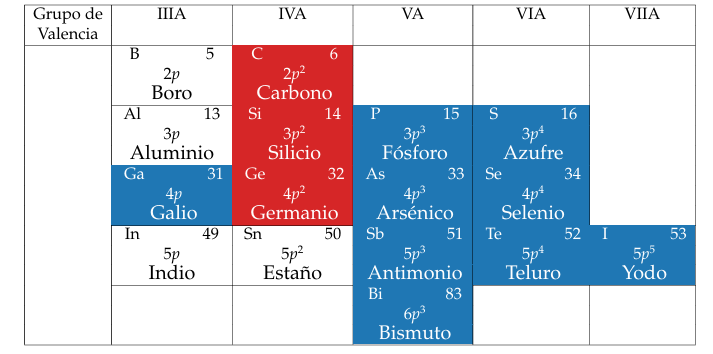
\includegraphics[width=0.8\textwidth]{../figures/Auxiliar_2_8.png}
        \caption{Extracto de la tabla periódica. Los átomos de Boro son del grupo IIIA, por lo tanto son átomos aceptores de electrones, mientras que los átomos de fósforo son del grupo VA y son átomos donadores de electrones.}
        \label{fig:tabla_periodica}
    \end{figure}
\end{frame}
%-------------------------
\begin{frame}
  
    \begin{figure}[H]
        \centering
        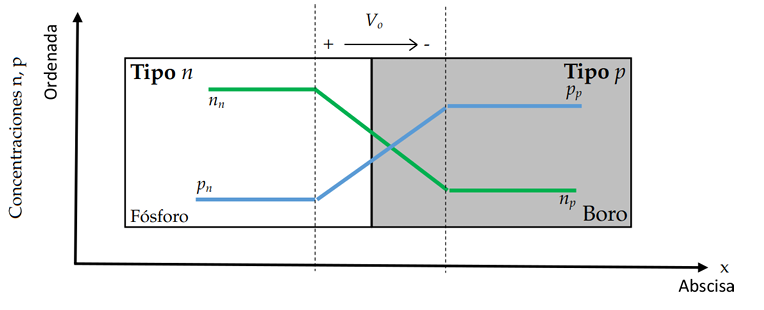
\includegraphics[width=0.8\textwidth]{../figures/Auxiliar_2_9}
        \caption{Perfiles de concentración de portadores en una unión p-n. La línea verde representa la concentración de electrones en función del espacio $n(x)$, mientras que la línea azul representa la concentración de huecos en función del espacio $p(x)$. Se observa la transición gradual en la región de depleción entre las regiones tipo n y tipo p.}
        \label{fig:concentraciones_pn}
    \end{figure}
\end{frame}
%------------------
\begin{frame}
    \begin{figure}[H]
        \centering
        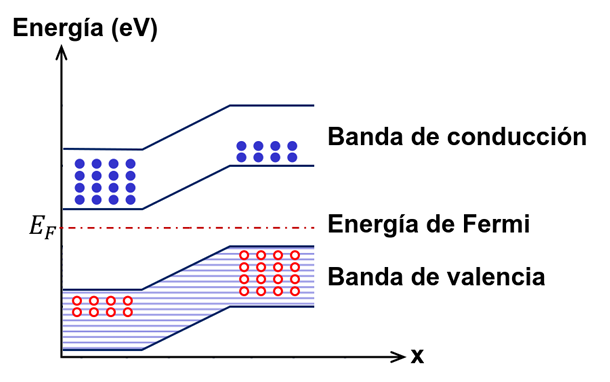
\includegraphics[width=0.6\textwidth]{../figures/Auxiliar_2_10}
        \caption{Diagrama de bandas de energía para una unión p-n en equilibrio térmico. Se muestran la banda de conducción, la banda de valencia, y la energía de Fermi ($E_F$). Los círculos azules representan electrones y los círculos rojos representan huecos. La curvatura de las bandas en la región de depleción crea una barrera de potencial.}
        \label{fig:bandas_pn}
    \end{figure}
\end{frame}

%---------
\section{Ejercicio 5}
\begin{frame}{Enunciado 5}
\begin{columns}
  \begin{column}{0.55\textwidth}
    \begin{block}{Enunciado ejercicio 5}
      \scriptsize
      Para el mismo material del problema 3 ahora se ve que en la curva verde existe un cambio como se nota en la Figura \ref{fig:p5}:

      \begin{enumerate}
          \item ¿Qué pudo haber producido este cambio?
          \item Si conociera el valor del punto rojo, ¿podría estimar el valor de la variable que está produciendo el cambio?
          \item ¿Qué necesitaría conocer para estimar la densidad de corriente asociada a esta curva? ¿Cuál sería su expresión si tuviera conocido todo lo que requiere?
          \item Bosqueje un diagrama de energía para esta situación.
      \end{enumerate}
    \end{block}
  \end{column}
  
  \begin{column}{0.43\textwidth}
    \begin{figure}[H]
        \centering
        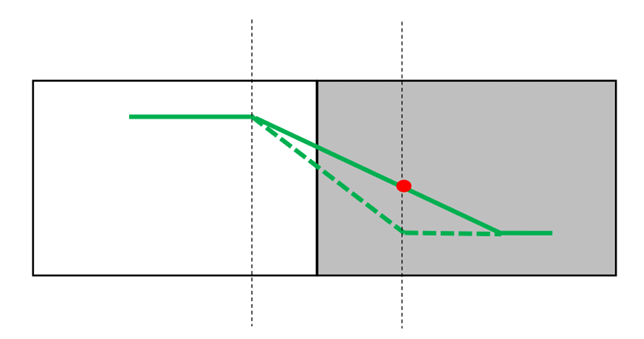
\includegraphics[width=\textwidth]{../figures/Auxiliar_2_2}
        \caption{Problema 5}
        \label{fig:p5}
    \end{figure}
  \end{column}
\end{columns}
\end{frame}
%------------------
\begin{frame}
    \begin{figure}[H]
        \centering
        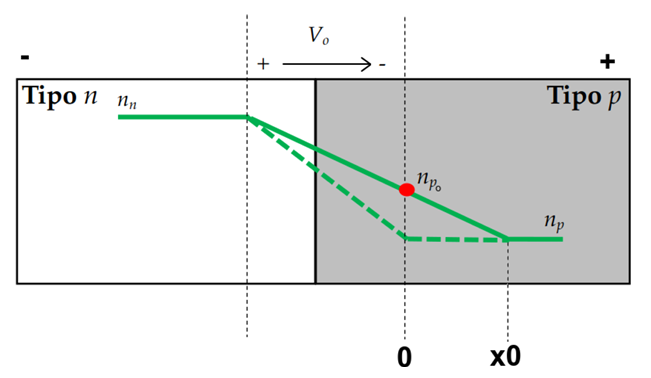
\includegraphics[width=0.7\textwidth]{../figures/Auxiliar_2_11}
        \caption{Voltaje externo aplicado con signo opuesto al voltaje de contacto $V_o$. Se observa cómo el perfil de concentración de electrones (línea verde sólida) se modifica comparado con el caso de equilibrio (línea verde punteada). El punto rojo indica la posición $x_0$ donde se produce el cambio más significativo.}
        \label{fig:voltaje_externo}
    \end{figure}
\end{frame}
%------------------
\begin{frame}
     \begin{figure}[H]
        \centering
        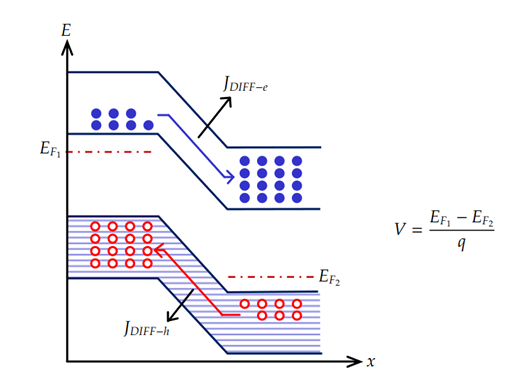
\includegraphics[width=0.5\textwidth]{../figures/Auxiliar_2_12}
        \caption{Diagrama de bandas de energía para una unión p-n bajo polarización directa. El voltaje externo cambia la estructura de la red cristalina, torciendo las bandas de energía. Los electrones del material tipo n ahora pueden moverse por difusión hacia el material tipo p, y a su vez, los huecos del material tipo p pueden moverse hacia el material tipo n. Esto se traduce en corrientes de difusión de electrones ($J_{\text{DIFF-e}}$) y de huecos ($J_{\text{DIFF-h}}$). Las diferencias entre las energías de Fermi dividida por la carga son equivalentes al voltaje externo.}
        \label{fig:bandas_polarizacion}
    \end{figure}
\end{frame}
\end{document}
